%%% PREAMBLE - Do not touch %%%%%%%%%%%%%%%%%%%%%%%%%%%%%%%%%%%%%%%%%%%%%%%%%%%%%%
\documentclass[10pt,twocolumn,letterpaper]{article}
\usepackage[ansinew]{inputenc}
\usepackage[portuguese,brazil,english]{babel}
\usepackage{model}
\usepackage{times}
\usepackage{epsfig}
\usepackage{graphicx}
\usepackage{amsmath}
\usepackage{amssymb}
\usepackage{color}
\usepackage{float}
\usepackage[pagebackref=true,breaklinks=true,letterpaper=true,colorlinks,bookmarks=false]{hyperref}

\cvprfinalcopy % *** Uncomment this line for the final submission
\def\httilde{\mbox{\tt\raisebox{-.5ex}{\symbol{126}}}}
\ifcvprfinal\pagestyle{empty}\fi

\newcommand{\TODO}[1]{TODO: #1}
\newcommand{\CITEONE}[2]{\mbox{#1 \cite{#2}}}
\newcommand{\CITETWO}[3]{\mbox{#1 and #2 \cite{#3}}}
\newcommand{\CITEN}[2]{\mbox{#1 et al. \cite{#2}}}

%%% Paper beginning %%%%%%%%%%%%%%%%%%%%%%%%%%%%%%%%%%%%%%%%%%%%%%%%%%%%%%%%%%%%%%
\begin{document}

%%% Title and authors %%%%%%%%%%%%%%%%%%%%%%%%%%%%%%%%%%%%%%%%%%%%%%%%%%%%%%%%%%%%
\title{MO444 Final Assignment - Beer Style Classification}
\author{Pedro Henrique M. X. Zacarin\thanks{\textbf{Contact}: \tt\small{phzacarin@gmail.com}}\\
}

%%% Abstract %%%%%%%%%%%%%%%%%%%%%%%%%%%%%%%%%%%%%%%%%%%%%%%%%%%%%%%%%%%%%%%%%%%%%
\maketitle
\begin{abstract}
In this project, a dataset with nearly $75000$ homemade beer recipes was utilized in order to train a beer style classifier. The dataset contains data of $170$ different beer styles with a total of $5$ useful features and is heavily imbalanced in its examples-per-class quantities. Allied to the fact that many beer styles shares common attributes, classification may be difficult and may not provide great accuracy results.
\end{abstract}

%%% Introduction %%%%%%%%%%%%%%%%%%%%%%%%%%%%%%%%%%%%%%%%%%%%%%%%%%%%%%%%%%%%%%%%%
\section{Introduction}
The production of homemade beers was always something important between the drink lovers. Many prefer making its own beer due to a set of reasons, such as spending less money with industrialized ones, picking specific ingredients, appeal to certain groups of people with different tastes or just for experimentation, to make something new.

The Internet has helped homebrewers's community a lot, as it enabled recipes and manufacturing techniques sharing and the opportunity to buy and sell different, and many times exotics and imported, ingredients. Furthermore, it allowed beer lovers to learn more about the production process, first steps, materials, ingredients and more intricate subjects involving chemistry and ingredient interaction.

Each beer has its style, which is a therm used to differentiate and categorize them by various factors such as color, appearance, production method, alcoholic content, origin or even history. There is a long list of styles, ranging from classic ones such as Bock, Altbier and Pale Ale to specialty styles such as Fruit Beer and Honey Beer.

In the website Kaggle (www.kaggle.com, a popular data science website that offers a great number of datasets) a dataset of nearly $75000$ homebrewed beers of over $170$ different styles originally shared in the website Brewer's Friend (www.brewersfriend.com) was available in order to be utilized for analysis, classification or sheer curiosity. That dataset was utilized in this project in order to try to assess the correlation between the beers features and its styles by building a classifier that predicts the beer style based on its features.

%%% Add section %%%%%%%%%%%%%%%%%%%%%%%%%%%%%%%%%%%%%%%%%%%%%%%%%%%%%%%%%%%%%%%%%%
\section{Dataset}

The original dataset needed to have its information treated in order to be utilized. First, the features which didn't have important information for classification or that had a great amount of missing data were removed, such as priming method, pitch rate and priming amount. Then, all rows corresponding to an original gravity and final gravity measured in Plato (measurement of the concentration of dissolved solids in a brewery wort) were also removed, as the vastly majority of the examples in the dataset were measured in another scale: Specific Gravity. The final treatment was to eliminate all beer styles with just one example, as it wouldn't be possible to separate a training and test set with each having at least one example of every class.

After the treatment mentioned above, the final dataset contained $67768$ examples from $168$ distinct styles with $5$ features each that could be utilized in order to train the classifier: original gravity (OG), final gravity (FG), alcoholic content (ABV), bitterness (IBU) and color which are all important measures of the brewing process. The color feature was already encoded into a continuous scale known as SRM (Standard Research Method).
 

%%% Add section %%%%%%%%%%%%%%%%%%%%%%%%%%%%%%%%%%%%%%%%%%%%%%%%%%%%%%%%%%%%%%%%%%
\section{Proposed solutions}
As mentioned in prior sections, the dataset utilized is heavily imbalanced. To illustrate such characteristic, a histogram with the frequency of each style was generated (Figure ~\ref{fig:style_hist}).

\begin{figure}[H]
\begin{center}
	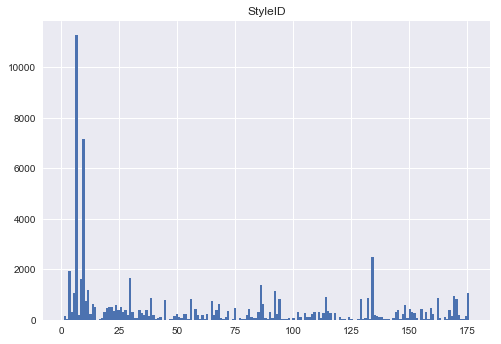
\includegraphics[width=0.4\textwidth]{pics/style_hist}
	\caption{Histogram showing style frequencies\label{fig:style_hist}}   
\end{center} 
\end{figure}   

The three most predominant styles have frequencies of $11270$ (American IPA), $7170$ (American Pale Ale) and $2466$ (Saison) examples each. It's worth noting that the $11270$ examples of American IPA style corresponds to roughly $1/6$ of all examples and the top $13$ most predominant styles corresponds together to half of all examples.

At first, the imbalance will be disregarded as an important characteristic and the whole dataset will be considered in order to attempt to train a classifier. A set of classification algorithms are going to be used to assess each one's resulting accuracy, with $80\%$ of the dataset for training and $20\%$ for cross validation. The algorithms are the following:

\begin{itemize}
	\item K-Nearest-Neighbors (K-NN)
	\item Support Vector Machines (SVMs) with One vs. One approach
	\item Random Forests (RF)
\end{itemize}

After each one of these methods were applied, a better approach will be considered: splitting the dataset into two, training the first one with the majority of the examples with one classifier and the other one, with classes with fewer examples, with another one. For that second scenario, a performance metric of 5x2 cross validation will be utilized.

\section{Development}
The first attempt made in order to create a classifier was to consider the whole dataset for the classification. The training set and test set were initially created considering the number of examples of each style, which leads to both sets preserving the percentage of samples for each class. For that scenario, $80\%$ of the dataset was utilized for training and $20\%$ for validation purposes.

K-Nearest-Neighbors is an algorithm utilized for both classification and regression based on feature similarity, where an object is classified by a majority vote of its neighbors, with the object being assigned to the class most common among its K nearest neighbors. To choose parameter K, grid search was performed (Table 1).

\begin{table}[h!]
  \begin{center}
    \label{tab:knn_table_whole}
    \begin{tabular}{c|c|c} % <-- Alignments: 1st column left, 2nd middle
      \textbf{K} & \textbf{Training accuracy ($\%$)} & \textbf{Validation accuracy ($\%$)}\\
      \hline
      10 & 39.93 & 30.46\\
      20 & 37.19 & 32.04\\
      30 & 36.11 & 32.43\\
      40 & 35.37 & 32.56\\
      50 & 34.86 & 32.59\\
      60 & 34.46 & 32.25\\
      70 & 34.14 & 32.36\\
      80 & 33.89 & 32.23\\
      90 & 33.58 & 32.00\\
      100 & 33.48 & 31.92\\
      150 & 32.75 & 31.86\\
    \end{tabular}
    \caption{Accuracies for each value of K in K-NN algorithm for whole dataset classification}
  \end{center}
\end{table}

K-Nearest-Neighbors algorithm resulted in training and cross validation accuracies of $34.86\%$  and $32.59\%$ respectively for K = $50$, which is far from a great result.

The next method applied was Support Vector Machines, which tries to find the best separation between classes by finding an hyperplane between the support vectors of each class considered. As the project's problem is multiclass, one vs. one approach was utilized, which means that comparisons between classes will be made two-by-two for every pair available. The training and validation accuracies obtained were respectively $39.12\%$ and $33.42\%$.

As a last try with the first scenario, Random Forest was utilized, which is an ensemble learning method for classification and regression that operate by constructing many decision trees at training time and utilizing bagging for generating them. Grid search was performed to assess the best number of estimators (number of trees in the forest) to be used (Table 2). The parameters for Random Forests algorithm were thoroughly tested in order to find the best combination avoiding overfitting, which are the following:

\begin{itemize}
	\item Number of features to be considered when looking for the best split: square root of the number of features
	\item Minimum number of samples required to split an internal node : $4$
	\item Maximum depth of the tree: $15$
\end{itemize}

In order to find a good number of estimators (trees in the forest), grid search was performed and the following results were obtained:

\begin{table}[h!]
  \begin{center}
    \label{tab:rf_table_whole}
    \begin{tabular}{c|c|c} % <-- Alignments: 1st column left, 2nd middle
      \textbf{N. estimators} & \textbf{Training accuracy ($\%$)} & \textbf{Validation accuracy ($\%$)}\\
      \hline
      50 & 57.88 & 35.92\\
      100 & 58.34 & 36.03\\
      200 & 58.44 & 35.92\\
      300 & 58.61 & 35.91\\
      400 & 58.60 & 35.93\\
      500 & 58.59 & 35.93\\
    \end{tabular}
    \caption{Accuracies for each number of estimators (trees) in Random Forests algorithm for whole dataset classification}
  \end{center}
\end{table}

As grid search shown, there is not a substantial difference between the number of estimators and validation accuracy, so $200$ was considered. With it, training and validation accuracies obtained were respectively $58.34\%$ and $36.03\%$.
 
In order to try to improve both training and validation accuracies, a split in the dataset was performed and each part of it was trained with a different method in order to mitigate, at least slightly, the effects of heavy class imbalance.

To find the best split for the original dataset (examples frequency threshold), grid search was utilized. For the first part of splitted dataset, which contains classes with more examples, Random Forests algorithm was used with $200$ estimators, as it was the one with better results in the previous scenario and because it works great with more examples. For the second part, which contains classes with fewer examples, SVMs with one vs. one approach and Random Forests will be employed to assess which one performs better in a case with fewer examples per class. A $80\%$ and $20\%$ separation between training and validation for each one of the parts from the original dataset was made. The results are displayed in Table 3 and Table 4.

\begin{table}[h!]
  \begin{center}
    \label{tab:freqs_splitted_first}
    \begin{tabular}{c|c|c} % <-- Alignments: 1st column left, 2nd middle
      \textbf{Split frequency} & \textbf{Examples (1st half)} & \textbf{Classes (1st half)}\\
      \hline
      200 & 61767 & 79\\
      300 & 56949 & 59\\
      400 & 50943 & 41\\
      500 & 46504 & 31\\
      550 & 44967 & 28\\
      600 & 43791 & 26\\
      650 & 41909 & 23\\
      750 & 40420 & 21\\
      800 & 39631 & 20\\
      850 & 35464 & 15\\
      900 & 33729 & 13\\
      950 & 31885 & 11\\
    \end{tabular}
    \caption{Number of examples and number of classes in first part of the splitted dataset for each frequency point of split}
  \end{center}
\end{table}

\begin{table}[h!]
  \begin{center}
    \label{tab:rf_splitted_first}
    \begin{tabular}{c|c|c} % <-- Alignments: 1st column left, 2nd middle
      \textbf{Split frequency} & \textbf{Tr. accuracy ($\%$)} & \textbf{Val. accuracy ($\%$)}\\
      \hline
      200 & 60.81 & 39.58\\
      300 & 63.30 & 41.81\\
      400 & 65.68 & 45.77\\
      500 & 67.87 & 49.30\\
      550 & 68.70 & 49.15\\
      600 & 69.44 & 50.16\\
      650 & 70.03 & 52.45\\
      750 & 71.82 & 53.83\\
      800 & 72.27 & 55.04\\
      850 & 74.57 & 60.05\\
      900 & 75.81 & 61.13\\
      950 & 76.58 & 63.43\\
    \end{tabular}
    \caption{Accuracies for each examples frequency split, with Random Forests being applied to the first part of the dataset with more examples per class}
  \end{center}
\end{table}

The results shown something that was already expected: the fewer classes in the first half dataset, the better the training and validation accuracy utilizing Random Forests. In order to find a sweet spot, it is necessary to run SVMs and Random Forests algorithms for the second half for the same frequency splits. The results can be seen in Table 6 and Table 7.

\begin{table}[h!]
  \begin{center}
    \label{tab:freq_splitted_second}
    \begin{tabular}{c|c|c} % <-- Alignments: 1st column left, 2nd middle
      \textbf{Split frequency} & \textbf{Examples (2nd half)} & \textbf{Classes (2nd half)}\\
      \hline
      200 & 6001 & 81\\
      300 & 10819 & 109\\
      400 & 16825 & 127\\
      500 & 21254 & 137\\
      550 & 22801 & 140\\
      600 & 23977 & 142\\
      650 & 25859 & 145\\
      750 & 27348 & 147\\
      800 & 28137 & 148\\
      850 & 32304 & 153\\
      900 & 34039 & 155\\
      950 & 35883 & 157\\
    \end{tabular}
    \caption{Number of examples and number of classes in first part of the splitted dataset for each frequency point of split}
  \end{center}
\end{table}

\begin{table}[h!]
  \begin{center}
    \label{tab:svms_splitted_second}
    \begin{tabular}{c|c|c} % <-- Alignments: 1st column left, 2nd middle
      \textbf{Split frequency} & \textbf{Tr. accuracy ($\%$)} & \textbf{Val. accuracy ($\%$)}\\
      \hline
      200 & 41.96 & 21.39\\
      300 & 41.59 & 25.50\\
      400 & 38.57 & 23.45\\
      500 & 36.08 & 23.39\\
      550 & 35.97 & 23.85\\
      600 & 35.38 & 24.83\\
      650 & 35.69 & 23.39\\
      750 & 35.54 & 24.07\\
      800 & 35.08 & 24.65\\
      850 & 35.75 & 25.65\\
      900 & 35.15 & 25.11\\
      950 & 34.20 & 23.69\\
    \end{tabular}
    \caption{Accuracies for each examples frequency split, with SVMs (one vs. one) being applied to the second part of the dataset with fewer examples per class}
  \end{center}
\end{table}

\begin{table}[h!]
  \begin{center}
    \label{tab:rf_splitted_second}
    \begin{tabular}{c|c|c} % <-- Alignments: 1st column left, 2nd middle
      \textbf{Split frequency} & \textbf{Tr. accuracy ($\%$)} & \textbf{Val. accuracy ($\%$)}\\
      \hline
      200 & 72.81 & 26.48\\
      300 & 68.56 & 30.22\\
      400 & 67.93 & 28.62\\
      500 & 65.58 & 26.99\\
      550 & 63.75 & 27.47\\
      600 & 62.26 & 27.90\\
      650 & 62.07 & 27.82\\
      750 & 60.80 & 28.26\\
      800 & 60.36 & 28.75\\
      850 & 60.58 & 30.15\\
      900 & 61.08 & 29.12\\
      950 & 60.62 & 28.06\\
    \end{tabular}
    \caption{Accuracies for each examples frequency split, Random Forests being applied to the second part of the dataset with fewer examples per class}
  \end{center}
\end{table}

The results from Tables 6 and 7 show that Random Forests are a better approach even for the second part of the dataset with fewer examples per class. Considering those results and the probability of an example to fall in the first or second part of the splitted original dataset, final training and validation accuracies were obtained, as may be seen in Table 8. 

\begin{table}[h!]
  \begin{center}
    \label{tab:final_accs_splitted}
    \begin{tabular}{c|c|c} % <-- Alignments: 1st column left, 2nd middle
      \textbf{Split frequency} & \textbf{Tr. accuracy ($\%$)} & \textbf{Val. accuracy ($\%$)}\\
      \hline
      200 & 61.87 & 38.41\\
      300 & 64.14 & 39.96\\
      400 & 66.24 & 41.51\\
      500 & 67.14 & 42.29\\
      550 & 67.03 & 41.85\\
      600 & 66.90 & 42.28\\
      650 & 67.00 & 43.05\\
      750 & 67.37 & 43.51\\
      800 & 67.32 & 44.12\\
      850 & 67.90 & 45.80\\
      900 & 68.41 & 45.05\\
      950 & 68.13 & 44.70\\
    \end{tabular}
    \caption{Final training and validation accuracies for each examples frequency split utilizing Random Forests in each part of the splitted dataset separately}
  \end{center}
\end{table}

The best split was in $850$, which cut the original dataset in two parts: one with $35464$ examples divided into $15$ classes and another with $32304$ examples divided into $153$ classes. Weighted training and validation accuracies were $67.9\%$ and $45.8\%$.

\section{Discussion}
%%%Talk about the experiments carried out and the obtained results. 

The first approach to the problem was to run a series of classification algorithms for the whole dataset, which resulted in training and validation accuracies of $34.86\%$  and $32.59\%$ for K-Nearest Neighbors, $39.12\%$ and $33.42\%$ for one vs. one SVMs and  $58.34\%$ and $36.03\%$ for Random Forests. The best results were given by Random Forests algorithm, showing a significant difference between them, which characterizes as overfitting of the training data even when the algorithm's parameters were tweaked to prevent this issue. Moreover, the validation accuracy was far from a good result.

For the second approach, an ensemble take was applied by dividing the original dataset into two: one with classes containing a higher number of examples and other with classes containing fewer examples. The first set contained $35464$ examples divided into $15$ classes and the second $32304$ examples divided into $153$ classes. Random Forests were utilized in the first one, as it was the algorithm with better performance for the whole dataset, and tends to do better with more examples. For the second, a comparison between performances of one vs. one SVMs and Random Forests was made, with the latter having an overall better performance. Based on the probability of an example to fit in the first or the second set, the final accuracies were calculated for the ensemble: $67.9\%$ and $45.8\%$ for training and validation, respectively, which was a substantial improvement over the first approach but still fell short of even a satisfatory result.

The low accuracies, particularly the validation one, could be explained by a series of factors. The dataset didn't have any truly distinctive feature and almost all of them showed ranges of values that could fit in a great number of classes, reducing the probability of a good classification. Moreover, the imbalance of classes even with the second approach was still present and affected classification, specially for the second portion of the dataset which had a good number of classes with very few examples (less than $50$), with the edge case being only $2$ examples.

The hypothesis of an overall bad dataset is also enforced when looking to the results of the first portion's classification, where only $15$ classes were present, with a great number of examples each (ranging from $862$ to $11270$), and even in this scenario classification results were modest: $74.57\%$ for training and $60.05\%$ for validation.
 
\section{Conclusion}
Even with two different approaches to the problem utilizing powerful multiclass classification algorithms the final results were below expected, which may be explained by the heavily imbalanced dataset and the nature of the features, which doesn't have many distinctions between them to characterize well most classes.


%%% References %%%%%%%%%%%%%%%%%%%%%%%%%%%%%%%%%%%%%%%%%%%%%%%%%%%%%%%%%%%%%%%%%%%



\end{document}